\section{eo\-Distribution$<$ EOT $>$ Class Template Reference}
\label{classeo_distribution}\index{eoDistribution@{eoDistribution}}
Abstract class for Distribution Evolution Algorithms within {\bf EO}{\rm (p.\,\pageref{class_e_o})}: the distribution itself.  


{\tt \#include $<$eo\-Distribution.h$>$}

Inheritance diagram for eo\-Distribution$<$ EOT $>$::\begin{figure}[H]
\begin{center}
\leavevmode
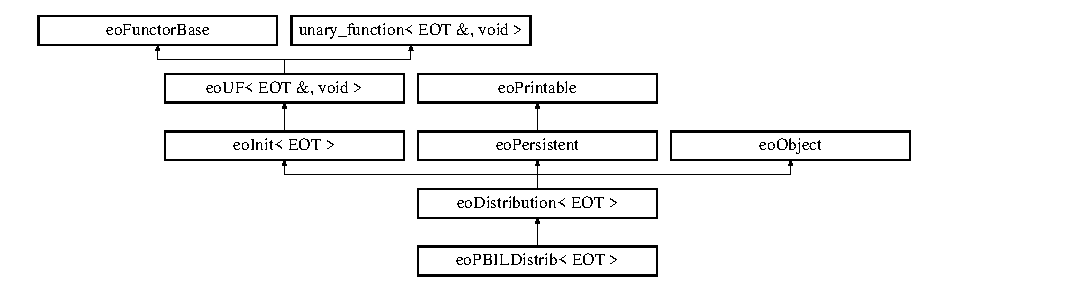
\includegraphics[height=3.48259cm]{classeo_distribution}
\end{center}
\end{figure}
\subsection*{Public Member Functions}
\begin{CompactItemize}
\item 
virtual void {\bf operator()} ({\bf EOT} \&)=0\label{classeo_distribution_a0}

\begin{CompactList}\small\item\em The pure virtual function that needs to be implemented by the subclass. \item\end{CompactList}\end{CompactItemize}


\subsection{Detailed Description}
\subsubsection*{template$<$class EOT$>$ class eo\-Distribution$<$ EOT $>$}

Abstract class for Distribution Evolution Algorithms within {\bf EO}{\rm (p.\,\pageref{class_e_o})}: the distribution itself. 

It basically IS AN {\bf eo\-Init}{\rm (p.\,\pageref{classeo_init})} - {\bf operator()(EOT \&)}{\rm (p.\,\pageref{classeo_distribution_a0})} generates new indis

The instances will probably be {\bf eo\-Value\-Param}{\rm (p.\,\pageref{classeo_value_param})} of some kind see {\bf eo\-PBILDistrib.h}{\rm (p.\,\pageref{eo_p_b_i_l_distrib_8h})} 



Definition at line 45 of file eo\-Distribution.h.

The documentation for this class was generated from the following file:\begin{CompactItemize}
\item 
eo\-Distribution.h\end{CompactItemize}
